%%%%%%%%%%%%%%%%%%%%%%%%%%%%%%%%%%%%%%%%%%%%%%%%%%%%%%%%
%%%%%%%%%%%%%%%%%%%%%%%%%%%%%%%%%%%%%%%%%%%%%%%%%%%%%%%%
%%%%%%%%%%%%%%%%%%%%%%%%%%%%%%%%%%%%%%%%%%%%%%%%%%%%%%%%
\chapter{Statistics}
\label{chap:stats}

%%%%%%%%%%%%%%%%%%%%%%%%%%%%%%%%%%%%%%%%%%%%%%%%%%%%%%%%
%%%%%%%%%%%%%%%%%%%%%%%%%%%%%%%%%%%%%%%%%%%%%%%%%%%%%%%%
\section{Expectation Value and Variance}
\label{stats:expval_and_var}

The expectation value \cref{eq:stats:exp_relations} and variance \cref{eq:stats:var_relations} are introductory, yet essential, statistical measures.
Their definitions and interesting properties are reproduced here for reference.
Note that $s$ is the unbiased sample variance,
the sample mean $\bar{x}$ has $\mu_{\bar{x}} = \mu$,
and the standard error is $\sigma_{\bar{x}} = \sigma / \sqrt{n}$,
where $\mu$ and $\sigma$ are from the parent population.

\begin{subequations}\label{eq:stats:exp_relations}
\begin{align}
\expvalE{X} = \expval{X} &= \sum_{j=1}^{m} x_{j} \, p_{j} = \int_{-\infty}^{\infty} x f\left(x\right) \, \dd{x} \label{eq:stats:exp_relations:def} \\
\bar{x} = \mu &= \frac{1}{n} \sum_{j=1}^{m} x_{j}\,,\,\text{for uniform}~p_{j} \label{eq:stats:exp_relations:mean} \\
\expval{X+Y} &= \expval{X} + \expval{X} \label{eq:stats:exp_relations:add} \\
\expval{a X} &= a \expval{X} \label{eq:stats:exp_relations:mult} \\
\expval{a} &= a \,\, \implies \, \expval{\expval{X}} = \expval{X} \label{eq:stats:exp_relations:self} \\
\expval{X Y}^{2} &\leq \expval{X^{2}} \expval{Y^{2}} \label{eq:stats:exp_relations:cbs_ineq}
\end{align}
\end{subequations}

\begin{subequations}\label{eq:stats:var_relations}
\begin{align}
\sigma_{X}^{2} = \variance{X} &= \expval{\left(x-\expval{x}\right)^{2}} = \expval{X^{2}} - \expval{X}^{2} \label{eq:stats:var_relations:def} \\
s^{2} &= \frac{1}{n-1} \sum_{j=1}^{m} \left( x_{j} - \expval{x}\right)^{2} \label{eq:stats:var_relations:sample} \\
s_{\bar{x}} &= \frac{s}{\sqrt{n}} \label{eq:stats:var_relations:standard_error_of_mean} \\
\variance{X+a} &= \variance{X} \label{eq:stats:var_relations:add} \\
\variance{a X} &= a^{2} \, \variance{X} \label{eq:stats:var_relations:mult} \\
\variance{a X \pm b Y} &= a^{2} \, \variance{X} + b^{2} \, \variance{Y} \pm 2 \, ab \, \cov{X}{Y} \label{eq:stats:var_relations:linear} \\
\variance{X \mid Y} &= \expval{\left(X - \expval{X \mid Y}\right)^{2} \mid Y} \label{eq:stats:var_relations:conditional1} \\
\variance{X} &= \expval{\variance{X \mid Y}} + \variance{\expval{X \mid Y}} \label{eq:stats:var_relations:conditional2}
\end{align}
\end{subequations}

%%%%%%%%%%%%%%%%%%%%%%%%%%%%%%%%%%%%%%%%%%%%%%%%%%%%%%%%
%%%%%%%%%%%%%%%%%%%%%%%%%%%%%%%%%%%%%%%%%%%%%%%%%%%%%%%%
\section{Covariance and Correlation}
\label{stats:corr_covar}

%%%%%%%%%%%%%%%%%%%%%%%%%%%%%%%%%%%%%%%%%%%%%%%%%%%%%%%%
\subsection{Covariance}
\label{stats:corr_covar:covariance}

The covariance between two variables $u$ and $v$,

\begin{equation}\label{eq:stats:covar}
\begin{split}
\sigma_{u,v}^{2} = \cov{u}{v} &= \frac{1}{m}\sum_{j=1}^{m}\left(u_{j}-\expval{u}\right)\left(v_{j}-\expval{v}\right) \\
&= \expval{\left(u-\expval{u}\right)\left(v-\expval{v}\right)} \\
&= \expval{u v} - \expval{u}\expval{v}\,,
\end{split}
\end{equation}

\noindent is a measure of their joint variability,
\ie a measure of any linear relationship which may exist between them.
It is helpful to remember the following covariance relations:

\begin{subequations}\label{eq:stats:covar_relations}
\begin{align}
\cov{X}{X} &= \variance{X}, \label{eq:stats:covar_relations:var} \\
\cov{X + a}{Y + b} &= \cov{X}{Y}, \label{eq:stats:covar_relations:add} \\
\cov{a\,X}{b\,Y} &= ab\,\cov{X}{Y}, \label{eq:stats:covar_relations:mult} \\
\cov{X}{Y}^{2} &\leq \variance{X}\variance{Y}. \label{eq:stats:covar_relations:inequality}
\end{align}
\end{subequations}

%%%%%%%%%%%%%%%%%%%%%%%%%%%%%%%%%%%%%%%%%%%%%%%%%%%%%%%%
\subsection{Pearson Correlation}
\label{stats:corr_covar:pearson}

The Pearson correlation coefficient,

\begin{equation}\label{eq:stats:corr:pearson}
\rho_{u,v} = \corr{u}{v} = \frac{\sigma_{u,v}^{2}}{\sigma_{u}\sigma_{v}} = \frac{\cov{u}{v}}{\sigma_{u}\sigma_{v}}\,,
\end{equation}

\noindent is a convenient dimensionless version, normalized to $-1 \leq \rho \leq 1$.
Example distributions can be found in \cref{fig:stats:corr_ex:pearson}.

\begin{figure}
\centering
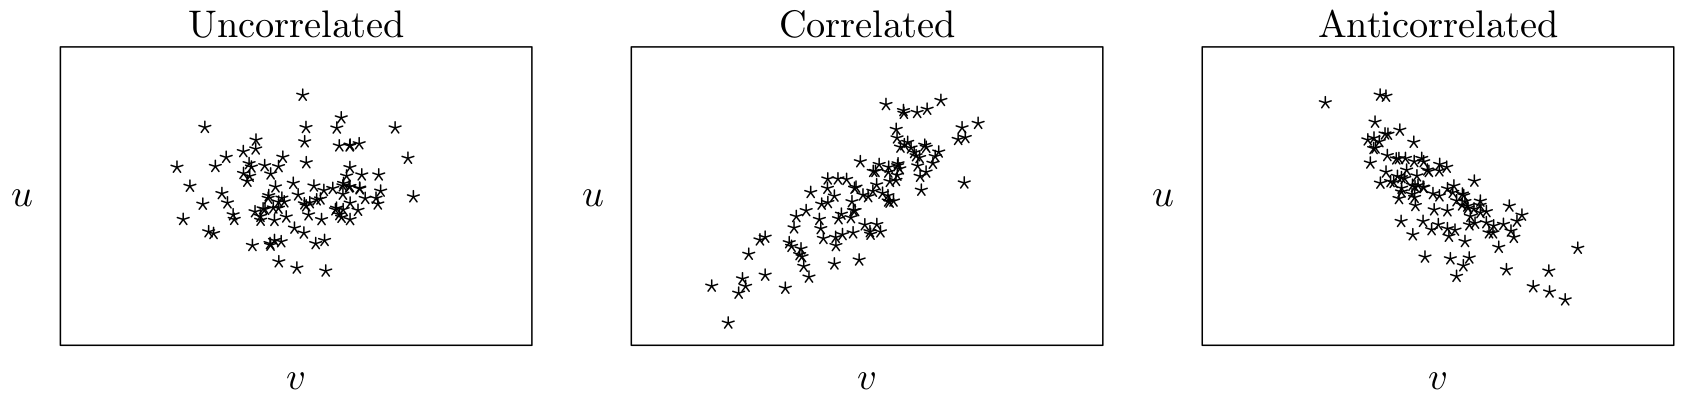
\includegraphics[width=0.95\textwidth]{figures/stats/corr_ex}
\caption{
Example distributions for
uncorrelated ($\rho \approx 0$),
correlated ($\rho \approx 1$),
and anticorrelated ($\rho \approx -1$)
variables $u$ and $v$ \cite{DougNotes}.
}
\label{fig:stats:corr_ex:pearson}
\end{figure}

%%%%%%%%%%%%%%%%%%%%%%%%%%%%%%%%%%%%%%%%%%%%%%%%%%%%%%%%
\subsection{Spearman Correlation}
\label{stats:corr_covar:spearman}

The Spearman rank correlation coefficient $r_{s}$ \cref{eq:stats:corr:spearman} is a non-parametric measure
used to quantify how well two variables are monotonically related,
\ie measure the degree of rank ordering between two variables across the available data points.
In contrast to the Pearson correlation coefficient,
a linear relationship between the variables is not assumed,
only that they increase or decrease in a consistent manner.
The Spearman correlation is simply the Pearson correlation of the variable's ranks,
where the rank function $R\left(x_{i}\right)$ returns the order,
$1, 2, 3, \ldots, m$, of a data point $x_{i}$ after being sorted\footnote{Ties
can be handled via dense ranking $1,2,2,3$, fractional ranking $1,2.5,2.5,4$, or arbitrarily broken with ordinal ranking $1,2,3,4$, \ie row numbering.}.
A comparison to the Pearson correlation coefficient can be found in \cref{fig:stats:corr_ex:spearman}.

\begin{equation}\label{eq:stats:corr:spearman}
r_{s} = \rho_{R\left(u\right),R\left(v\right)} = \frac{\cov{R\left(u\right)}{R\left(v\right)}}{\sigma_{R\left(u\right)}\sigma_{R\left(v\right)}}\,.
\end{equation}

\begin{figure}[H]
  \centering
  \begin{subfigure}[c]{0.48\textwidth}\centering
    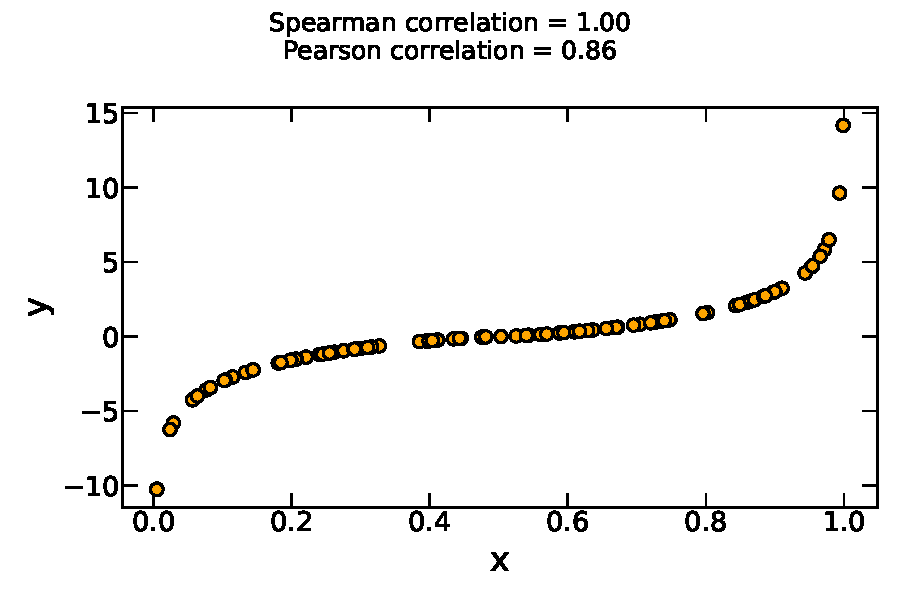
\includegraphics[width=\textwidth]{figures/stats/spearman_corr_non_para}
  \caption{Non-Parametric}
  \label{fig:stats:corr_ex:spearman:non_para}
  \end{subfigure}
  ~
  \begin{subfigure}[c]{0.48\textwidth}\centering
    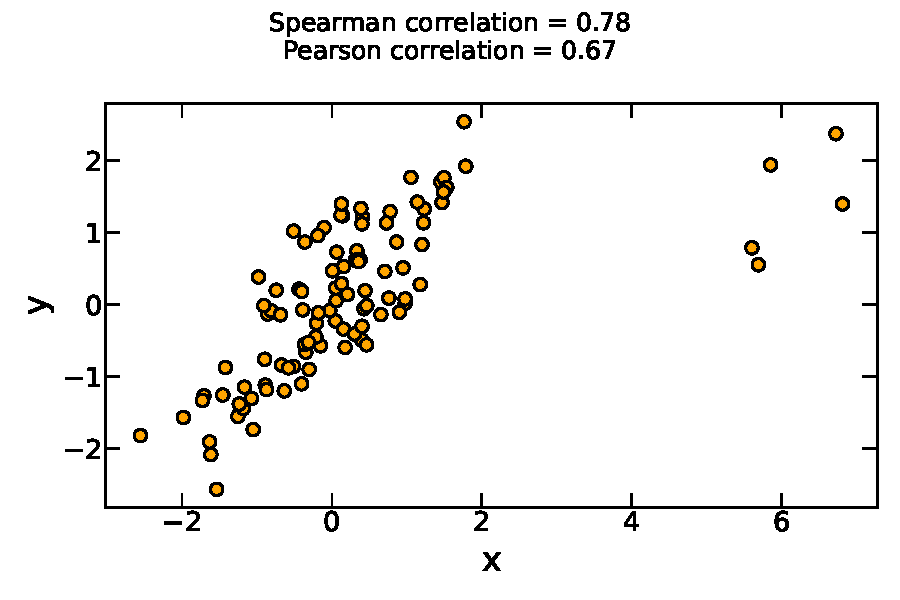
\includegraphics[width=\textwidth]{figures/stats/spearman_corr_outliers}
  \caption{Outliers}
  \label{fig:stats:corr_ex:spearman:outliers}
  \end{subfigure}
\caption{
Comparisons of the Spearman rank correlation and Pearson correlation coefficients,
adapted from
\href{https://en.wikipedia.org/wiki/File:Spearman_fig1.svg}{Skbkekas} and
\href{https://en.wikipedia.org/wiki/File:Spearman_fig3.svg}{Skbkekas}.
Note that non-parametric Spearman rank correlation
only measures the monotonic nature of the data, not its linearity,
and is more resilient to outliers.
\label{fig:stats:corr_ex:spearman}
}
\end{figure}

%%%%%%%%%%%%%%%%%%%%%%%%%%%%%%%%%%%%%%%%%%%%%%%%%%%%%%%%
\subsection{Covariance Matrix}
\label{stats:corr_covar:covar_matrix}

The covariance matrix,

\begin{align}\label{eq:covar_matrix}
  \mb{M} = \begin{pmatrix}
    \sigma_{1}^2 & \cov{1}{2}   & \cov{1}{3}   & \ldots \\
    \cov{1}{2}   & \sigma_{2}^2 & \cov{2}{3}   & \ldots \\
    \cov{1}{3}   & \cov{2}{3}   & \sigma_{3}^2 & \ldots \\
    \vdots       & \vdots       & \vdots       & \ddots
  \end{pmatrix}\,,
\end{align}

\noindent with elements $M_{ij} = \expval{\left(u_{i} - \expval{u}_{i}\right)\left(u_{j}-\expval{u}_{j}\right)}$
is the higher dimensional extension of the covariance.
We can visualize the covariance between variables with
Gaussian error ellipses given by the probability distribution

\begin{equation}\label{eq:stats:P_error_ellipse_k}
P\left(x_{1},x_{2},\ldots,x_{k}\right) = \frac{1}{(2\pi)^{k/2}}\frac{1}{\abs{\mb{M}}^{1/2}}\exp\left[-\frac{1}{2}\left(\vb{x}-\vb*{\mu}\right)^{\transpose}\mb{M}\left(\vb{x}-\vb*{\mu}\right)\right]\,,
\end{equation}

\noindent where the ellipse semi-axes are directed along the eigenvectors of $\mb{M}$.
In two dimensions it is easier to see the equation of the error ellipse itself:

\begin{equation}\label{eq:stats:P_error_ellipse_2}
\begin{split}
P\left(u,v\right) &= \frac{1}{2\pi\sigma_{u}\sigma_{v}}\frac{1}{\sqrt{1-\rho^{2}}}\exp\bigg\{-\frac{1}{2}\bigg[ \\
&\frac{1}{(1-\rho)^{2}}\left(\frac{\left(u-\expval{u}\right)^{2}}{\sigma_{u}^{2}}+\frac{\left(v-\expval{v}\right)^{2}}{\sigma_{v}^{2}}-\frac{2\rho \left(u-\expval{u}\right)\left(v-\expval{v}\right)}{\sigma_{u}\sigma_{v}}\right)\bigg]\bigg\}\,.
\end{split}
\end{equation}

%%%%%%%%%%%%%%%%%%%%%%%%%%%%%%%%%%%%%%%%%%%%%%%%%%%%%%%%
%%%%%%%%%%%%%%%%%%%%%%%%%%%%%%%%%%%%%%%%%%%%%%%%%%%%%%%%
\section{Central Limit Theorem (CLT)}
\label{stats:CLT}

The central limit theorem (CLT) states that
if we take samples of size $n$ from an independent random variable multiple times,
from any distribution\footnote{Where the mean is defined, \ie not the Cauchy or other pathological distributions.},
the sample means will tend to the normal distribution.
In practice, we typically require $\num{30} \lesssim n$ points per sample before we say the CLT applies.
The CLT is an important result in statistics as it lets us
treat many problems in a normally distributed framework,
in particular finding confidence intervals for the sample mean,
and hypothesis testing for sample means with a \ttest or ANOVA.

%%%%%%%%%%%%%%%%%%%%%%%%%%%%%%%%%%%%%%%%%%%%%%%%%%%%%%%%
%%%%%%%%%%%%%%%%%%%%%%%%%%%%%%%%%%%%%%%%%%%%%%%%%%%%%%%%
\section{Bayes' Theorem}
\label{stats:Bayes_rule}

Bayes' theorem follows from the probability of the intersection of two events $A$ and $B$:

\begin{equation}\label{eq:stats:intersection}
P\left(A \cap B\right) = P\left(A \mid B\right) P\left(B\right) = P\left(B \mid A\right) P\left(A\right).
\end{equation}

\noindent Dividing by $P\left(B\right)$ we have:

\begin{equation}\label{eq:stats:Bayes_rule}
\begin{split}
P\left(A \mid B\right) &= \frac{P\left(B \mid A\right) P\left(A\right)}{P\left(B\right)}\,, \\
&= \frac{P\left(B \mid A_{i}\right) P\left(A_{i}\right)}{\sum_{j} P\left(B \mid A_{j}\right)P\left(A_{j}\right)}\,, \\
\text{Posterior} &= \frac{\text{Likelihood} \times \text{Prior}}{\text{Normalization}}\,.
\end{split}
\end{equation}

\subsubsection{Example: Medical Testing}
\label{stats:Bayes_rule:medical_test}

Example: Testing for disease with a \SI{2}{\percent} incidence rate in the wider population.
The test has a \SI{99}{\percent} true positive rate and a \SI{5}{\percent} false positive rate.
What is the probability an individual has the disease if their test is positive?

% https://www.wolframalpha.com/input/?i=(0.99*0.02)%2F((0.99*0.02)%2B(0.05*(1%E2%88%920.02)))
\begin{equation}\label{eq:stats:Bayes_rule:medical_test_1}
\begin{split}
P\left(\text{Infected} \mid +\right) &= \frac{P\left(+ \mid \text{Infected}\right) P\left(\text{Infected}\right)}{P\left(+\right)}\,, \\
 &= \frac{P\left(+ \mid \text{Infected}\right) P\left(\text{Infected}\right)}{
P\left(+ \mid \text{Infected}\right)P\left(\text{Infected}\right) + P\left(+ \mid \text{Healthy}\right)P\left(\text{Healthy}\right)}\,, \\
&= \frac{\num{0.99} \times \num{0.02}}{\num{0.99} \times \num{0.02} + \num{0.05} \times \left(1-\num{0.02}\right)}\,, \\
&\approx \num{0.288}\,.
\end{split}
\end{equation}

\noindent And if we then run a second, independent, test which also comes back positive?

% https://www.wolframalpha.com/input/?i=(0.99*0.288)%2F((0.99*0.288)%2B(0.05*(1%E2%88%920.288)))
\begin{equation}\label{eq:stats:Bayes_rule:medical_test_2}
\begin{split}
P\left(\text{Infected} \mid ++\right) &= \frac{P\left(+ \mid \text{Infected}\right) P\left(\text{Infected} \mid +\right)}{
P\left(+ \mid \text{Infected}\right)P\left(\text{Infected} \mid +\right) + P\left(+ \mid \text{Healthy}\right)P\left(\text{Healthy} \mid +\right)}\,, \\
&= \frac{\num{0.99} \times \num{0.288}}{\num{0.99} \times \num{0.288} + \num{0.05} \times \left(1-\num{0.288}\right)}\,, \\
&\approx \num{0.889}\,.
\end{split}
\end{equation}

\noindent Note that if we ran both tests the first time we would still have:

% https://www.wolframalpha.com/input/?i=(0.99%5E2*0.02)%2F((0.99%5E2*0.02)%2B(0.05%5E2*(1%E2%88%920.02)))
\begin{equation}\label{eq:stats:Bayes_rule:medical_test_3}
\begin{split}
P\left(\text{Infected} \mid ++\right) &= \frac{P\left(++ \mid \text{Infected}\right) P\left(\text{Infected}\right)}{P\left(++\right)}\,, \\
&= \frac{\num{0.99}^{2} \times \num{0.02}}{\num{0.99}^{2} \times \num{0.02} + \num{0.05}^{2} \times \left(1-\num{0.02}\right)}\,, \\
&\approx \num{0.889}\,.
\end{split}
\end{equation}

\subsubsection{Example: Biased Coin}
\label{stats:Bayes_rule:biased_coin}

Consider the case of a bag of $n$ fair coins and $m$ biased coins.
Let $P\left(H \mid \stcomp{F}\right) \equiv p_{H}$ be the \apriori probability of heads $H$ for an biased coin $\stcomp{F}$.
Drawing one coin from the bag, you flip it multiple times recording $h$ heads and $t$ tails.
What is the probability you have drawn an biased coin, $P\left(\stcomp{F} \mid h,t\right)$?

\begin{equation}\label{eq:stats:Bayes_rule:biased_coin_setup}
\begin{gathered}
P\left(F\right) = \frac{n}{n+m}\,,\quad P\left(\stcomp{F}\right) = \frac{m}{n+m}\,, \\
P\left(H \mid F\right) = \frac{1}{2}\,,\quad P\left(h,t \mid F\right) = \left(\frac{1}{2}\right)^{h}\,\left(\frac{1}{2}\right)^{t} = \frac{1}{2^{h+t}}\,, \\
P\left(h,t \mid \stcomp{F}\right) = P\left(H \mid \stcomp{F}\right)^{h} P\left(\stcomp{H} \mid \stcomp{F}\right)^{t} = p_{H}^{h} \left(1-p_{H}\right)^{t}.
\end{gathered}
\end{equation}

\begin{equation}\label{eq:stats:Bayes_rule:biased_coin_solution}
\begin{split}
P\left(\stcomp{F} \mid h,t\right) &= \frac{
P\left(h,t \mid \stcomp{F}\right) P\left(\stcomp{F}\right)}{
P\left(h,t \mid \stcomp{F}\right) P\left(\stcomp{F}\right) + P\left(h,t \mid F\right) P\left(F\right)} \\
&= \frac{
m\,p_{H}^{h} \left(1-p_{H}\right)^{t}}{
m\,p_{H}^{h} \left(1-p_{H}\right)^{t} + n\,2^{-h-t}}\,.
\end{split}
\end{equation}

Some example values are provided in \cref{tab:Bayes_rule:biased_coin}.

\begin{table}[H]
\centering
\begingroup
\renewcommand*{\arraystretch}{1}
% $m = 50$, $n = 50$

\begin{tabular}{c c c c}
\hline
$h$ & $t$ & $p_{H}$ & $P\left(\stcomp{F} \mid h,t\right)$ \\
\hline
\hline
10 & 0 & 1.00 & 0.99902 \\
10 & 0 & 0.80 & 0.99099 \\
10 & 0 & 0.60 & 0.86095 \\
\hline
7 & 3 & 0.99 & 0.00095 \\
7 & 3 & 0.80 & 0.63208 \\
7 & 3 & 0.60 & 0.64722 \\
\hline
5 & 5 & 0.99 & 0.00000 \\
5 & 5 & 0.80 & 0.09696 \\
5 & 5 & 0.60 & 0.44915 \\
\hline
75 & 25 & 0.99 & 0.00000 \\
75 & 25 & 0.80 & 1.00000 \\
75 & 25 & 0.60 & 0.99970 \\
\hline
\end{tabular}
\endgroup
\caption{
$P\left(\stcomp{F} \mid h,t\right)$ for various values of $h$, $t$, and $p_{H}$ when $m = 50$, $n = 50$.
}
\label{tab:Bayes_rule:biased_coin}
\end{table}

%%%%%%%%%%%%%%%%%%%%%%%%%%%%%%%%%%%%%%%%%%%%%%%%%%%%%%%%
%%%%%%%%%%%%%%%%%%%%%%%%%%%%%%%%%%%%%%%%%%%%%%%%%%%%%%%%
\section{Coin Problems}
\label{stats:coin_problems}

%%%%%%%%%%%%%%%%%%%%%%%%%%%%%%%%%%%%%%%%%%%%%%%%%%%%%%%%
\subsection{Making an Biased Coin Fair}
\label{stats:coin_problems:biased_to_fair}
% https://fivethirtyeight.com/features/can-you-make-an-unfair-coin-fair/
% https://fivethirtyeight.com/features/can-you-snatch-defeat-from-the-jaws-of-victory/
% https://youtu.be/-SANBbv0-Hw
% https://math.stackexchange.com/a/146614 for additional references

If we are given an biased coin with $P\left(H\right) = p \neq \num{0.5}$
we can construct a fair coin\footnote{The solution is credited to John von Neumann, who really did work on everything!} by
flipping the biased coin $m$ times and selecting outcomes with an equal probability of occurring, while disregarding all other outcomes.
For example, with $m=2$ flips we have the outcomes listed in \cref{tab:coin_problems:biased_to_fair:m2_outcomes}:

\begin{table}[H]
\centering
\begingroup
\renewcommand*{\arraystretch}{1}
\begin{tabular}{c c c c}
\hline
Outcome & $P\left(\text{Outcome}\right)$ & Assignment \\
\hline
\hline
$HH$ & $p^{2}$ & Disregard \\
$HT$ & $p\left(1-p\right)$ & H \\
$TH$ & $\left(1-p\right)p$ & T \\
$TT$ & $\left(1-p\right)^{2}$ & Disregard \\
\end{tabular}

\endgroup
\caption{
Making an biased coin fair in $m=2$ flips.
}
\label{tab:coin_problems:biased_to_fair:m2_outcomes}
\end{table}

Note that we are disregarding $p^{2} + \left(1-p\right)^{2}$ percent of flips
and this method will become increasingly inefficient as $p$ moves away from $\num{0.5}$.
We can improve the efficiency by increasing $m$ and reassigning the
outcomes\footnote{For $m = \num{4}$, disregard $P\left(HHHH \parallel TTTT\right) = p^{4} + \left(1-p\right)^{4} < p^{2} + \left(1-p\right)^{2}$,\newline
$HT \parallel HHHT \parallel HHTT \parallel TTHT \to H$,\newline
$TH \parallel TTTH \parallel TTHH \parallel HHTH \to T = H^{-1}$.} such that
we decrease the average number of flips required.
If we need to simulate something with more outcomes, like a 6 sided die,
we can increase $m$ until we have enough equal outcomes, or combinations of outcomes.

We can also ask, for what values of $p$ is a fair outcome ensured in $m$ flips?
To solve, create $P\left(\text{Outcome}\right)$ for all possible outcomes of $m$ flips.
Then, sum all possible combinations\footnote{Excluding the combination with all outcomes where $\sum P\left(\text{Outcome}\right) = 1$.} of $P\left(\text{Outcome}\right)$
and try to solve $\sum P\left(\text{Outcome}\right) = \num{0.5}$.
This partitions the outcomes into two assignments without disregarding any outcomes, \ie no flips are wasted.
For example, with $m=2$ and \cref{tab:coin_problems:biased_to_fair:m2_outcomes}, we solve
$p^{2}$, $p\left(1-p\right)$, $\left(1-p\right)^{2}$,
$p^{2} + p\left(1-p\right)$, $p\left(1-p\right) + \left(1-p\right)^{2}$, and $p^{2} + \left(1-p\right)^{2} = \num{0.5}$
separately for $0<p<1$.
The valid $p$ are then
$p = 1/\sqrt{2}$ with $HH \to H$,
$p = \num{0.5}$ with $HH \parallel TT \to H$,
and $p = 1 - 1/\sqrt{2}$ with $TT \to H$;
everything else $\to T$.

%%%%%%%%%%%%%%%%%%%%%%%%%%%%%%%%%%%%%%%%%%%%%%%%%%%%%%%%
\subsection{Making an Fair Coin Biased}
\label{stats:coin_problems:fair_to_biased}

In the opposite direction, we can also make a fair coin biased
with $P\left(H\right) = p = 1/N$ by flipping it
$m = \text{ceil}\left(\log_{2}N\right)$ times
and reassigning the outcomes such that $H^{m} \to H$,
$N-1$ other outcomes $\to T$, and we disregard any remaining $m-N$ outcomes.

%%%%%%%%%%%%%%%%%%%%%%%%%%%%%%%%%%%%%%%%%%%%%%%%%%%%%%%%
%%%%%%%%%%%%%%%%%%%%%%%%%%%%%%%%%%%%%%%%%%%%%%%%%%%%%%%%
\section{Uniform Distribution}
\label{stats:uniform}

The uniform distribution, \cref{eq:stats:uniform:P} and \cref{fig:dist:uniform},
is the simplest probability distribution
having a constant probability $1/(b-a)$ over the interval $a$ to $b$.

\begin{equation}\label{eq:stats:uniform:P}
P\left(x;\,a,\,b\right) = \begin{cases}
\frac{1}{b-a} & a \leq x \leq b \,, \\
0 & \text{otherwise} \,,
\end{cases}
\end{equation}

It is illustrative to compute the mean and variance of the uniform distribution from $P(x)$ directly:

\begin{subequations}\label{eq:stats:uniform:mean_variance}
\begin{align}
\expval{x} &= \int_{-\infty}^{\infty} x P\left(x\right) \, \dd{x} = \frac{1}{b-a} \int_{a}^{b} x \, \dd{x} = \frac{1}{2(b-a)}\left(b^{2} - a^{2}\right) = \frac{1}{2}\left(a + b\right)\,, \label{eq:stats:uniform:mean_variance:mean} \\
\variance{x} &= \expval{x^{2}} - \expval{x}^{2} = \frac{1}{b-a} \int_{a}^{b} x^{2} \, \dd{x} - \expval{x}^{2} = \cdots = \frac{1}{12}\left(b-a\right)^{2}\,. \label{eq:stats:uniform:mean_variance:variance}
\end{align}
\end{subequations}

%%%%%%%%%%%%%%%%%%%%%%%%%%%%%%%%%%%%%%%%%%%%%%%%%%%%%%%%
%%%%%%%%%%%%%%%%%%%%%%%%%%%%%%%%%%%%%%%%%%%%%%%%%%%%%%%%
\section{Binomial Distribution}
\label{stats:binomial}

The binomial distribution, \cref{eq:stats:binomial:P} and \cref{fig:dist:binomial},
gives the probability of observing $k$ successes in $n$ independent Boolean trials,
when $p$ is the probability of success in any one trial.

\begin{subequations}\label{eq:stats:binomial}
\begin{align}
P\left(k;\,n,p\right) &= \binom{n}{k} p^{k} \left(1-p\right)^{n-k}, \label{eq:stats:binomial:P} \\
\binom{n}{k} &\equiv \frac{n!}{k!\left(n-k\right)!}\,. \label{eq:stats:binomial_coefficient}
\end{align}
\end{subequations}

\noindent Here \cref{eq:stats:binomial_coefficient} is the binomial coefficient,
representing the number of unordered combinations
which select $k$ elements from $n$ elements; $n$ choose $k$.

The mean and variance of the binomial distribution are:

\begin{subequations}\label{eq:stats:binomial:mean_variance}
\begin{align}
\expval{k} &= \sum_{k=0}^{n} k P\left(k;\,n,p\right) = n p\,, \label{eq:stats:binomial:mean} \\
\sigma^{2} &= n p\left(1-p\right). \label{eq:stats:binomial:variance}
\end{align}
\end{subequations}

\subsubsection{Bernoulli Distribution}
\label{stats:binomial:bernoulli}

For the special case when $n=1$, we have the Bernoulli distribution:

\begin{equation}\label{eq:stats:bernoulli}
P\left(k;\,p\right) = p^{k} \left(1-p\right)^{1-k}, \quad \expval{k} = p\,, \quad \sigma^{2} = p\left(1-p\right).
\end{equation}

\subsubsection{Negative Binomial Distribution}
\label{stats:binomial:negative}

If we are interested in the probability of
observing $k$ successes before we observe $r$ failures,
we can slightly modify the binomial distribution to be
the ``negative''\footnote{Negative as in $\binom{k+r-1}{k} = \left(-1\right)^{k} \binom{-r}{k}$.} binomial distribution:

\begin{subequations}\label{eq:stats:binomial:neg:P}
\begin{align}
P\left(k;\,r,p\right) = \binom{k+r-1}{k} p^{k} \left(1-p\right)^{r}\,,
\end{align}
\end{subequations}

\noindent where $p$ is still the probability of a success.
Note that since we stop on the $r^{\text{th}}$ failure,
we need to only arrange the $k$ successes in the first $k+r-1$ trials.

The mean and variance are then:

\begin{subequations}\label{eq:stats:binomial:neg:mean_variance}
\begin{align}
\expval{k} &= r p / \left(1-p\right)\,, \label{eq:stats:binomial:neg:mean} \\
\sigma^{2} &= r p / \left(1-p\right)^{2}. \label{eq:stats:binomial:neg:variance}
\end{align}
\end{subequations}

%%%%%%%%%%%%%%%%%%%%%%%%%%%%%%%%%%%%%%%%%%%%%%%%%%%%%%%%
%%%%%%%%%%%%%%%%%%%%%%%%%%%%%%%%%%%%%%%%%%%%%%%%%%%%%%%%
\section{Poisson Distribution}
\label{stats:poisson}

For rare processes with $p \ll 1$, and thus $\lambda \equiv n\,p \ll 1$,
the binomial distribution reduces\footnote{See
one \href{https://medium.com/@andrew.chamberlain/deriving-the-poisson-distribution-from-the-binomial-distribution-840cc1668239}{derivation here}.
In practice, $\num{20} \lesssim n$, $\lambda = n\,p \lesssim \num{10}$ is a reasonable standard.} to the
Poisson distribution:

\begin{equation}\label{eq:stats:poisson:P}
P\left(k;\,\lambda\right) = \frac{\lambda^{k}}{k!}\,e^{-\lambda}\,, \\
\end{equation}

\noindent where $\lambda$ is the expected number of events in a given interval,
$\lambda = \left(\text{event density}\right) \times \left(\text{interval}\right)$.
Note that $\lambda$ has dimensionless units of counts of events\footnote{Although
we are typically considering $\lambda$ events in a given time interval,
$\lambda_{\text{Poisson}}$ is not a rate, yet!} and does not have to be an integer.
When events occur independently and at a constant rate,
which is low enough that no events occur simultaneously within our measurement resolution,
the event count per time interval will follow the Poisson distribution.
Such a situation is known as a Poisson process.
A plot of the distribution can be found in \cref{fig:dist:poisson}.

Interestingly, the mean and variance of the Poisson distribution are identical and equal to $\lambda$:

\begin{equation}\label{eq:stats:poisson:mean_variance}
\expval{k} = \sigma^{2} = \lambda\,.
\end{equation}

%%%%%%%%%%%%%%%%%%%%%%%%%%%%%%%%%%%%%%%%%%%%%%%%%%%%%%%%
%%%%%%%%%%%%%%%%%%%%%%%%%%%%%%%%%%%%%%%%%%%%%%%%%%%%%%%%
\section{Exponential Distribution}
\label{stats:exp}

If we sample the time intervals between Poisson distributed events\footnote{Assuming the first event occurs at $T$,
$P\left(T > t\right) = P_{\text{Poisson}}\left(k=0;\,\lambda_{\text{Poisson}} \equiv \lambda\,t\right) = e^{-\lambda t}$,
$P\left(t\right) = \dv{t} P\left(T \leq t\right) = \dv{t} 1 - e^{-\lambda t} = \lambda e^{-\lambda t}$.
Here we have used the Poisson distribution to find the CDF,
then differentiated to find the PDF.
$\lambda$ is now a rate, unlike $\lambda_{\text{Poisson}}$!} we
arrive at the exponential distribution,

\begin{equation}\label{eq:stats:exp:P}
P\left(x;\,\lambda\right) = \begin{cases}
\lambda e^{-\lambda x} & x \geq 0 \,, \\
0 & x < 0 \,,
\end{cases}
\end{equation}

\noindent with rate parameter $\lambda$ events per unit $x$.
A plot of the distribution can be found in \cref{fig:dist:exp}.

The mean and standard deviation of the exponential distribution are identical and equal to $1/\lambda$:

\begin{equation}\label{eq:stats:exp:mean_variance}
\expval{x} = \sigma = \frac{1}{\lambda}\,, \quad \sigma^{2} = \frac{1}{\lambda^{2}}\,.
\end{equation}

The exponential distribution is memoryless\footnote{The exponential (geometric) distribution is the only real number (integer) memoryless probability distribution.} \cref{eq:stats:exp:memoryless},
\ie the time until a future event occurs does not depend on the time elapsed at the present.

\begin{equation}\label{eq:stats:exp:memoryless}
P\left(T > t + s \mid T > s\right) = P\left(T > t\right)\,, \quad \forall s,t \geq 0.
\end{equation}

%%%%%%%%%%%%%%%%%%%%%%%%%%%%%%%%%%%%%%%%%%%%%%%%%%%%%%%%
%%%%%%%%%%%%%%%%%%%%%%%%%%%%%%%%%%%%%%%%%%%%%%%%%%%%%%%%
\section{Example: Cars Driving By}
\label{stats:cars}

After watching a patch of road,
you notice that on average cars are spaced \SI{5}{\minute} apart.
Assume the cars are traveling independently\footnote{Not a good assumption
in real life as cars will clump up in traffic, \ie become correlated.
Better examples include
radioactive decay,
photon arrival from a distant star,
support tickets being created\ldots} of one another.

\subsubsection{Questions}
\label{stats:cars:questions}

\begin{enumerate}[noitemsep]
  \item What is $P\left(\text{Observing \num{5} cars in the next \SI{6}{\minute}}\right)$?\label{item:stats:cars:1}
  \item If \SI{20}{\percent} of the cars are red, what is $P\left(\text{Observing \num{5} red cars in the next \SI{6}{\minute}}\right)$?\label{item:stats:cars:2}
  \item What is $P\left(\text{Observing \num{2} or more cars in the next \SI{10}{\minute}}\right)$?\label{item:stats:cars:3}
  \item \num{100} cars have just driven by, how many are expected in the next hour?\label{item:stats:cars:4}
  \item If we start watching the road at a random time, how long should we expect to wait until we see our first car?\label{item:stats:cars:5}
\end{enumerate}

\subsubsection{Solutions}
\label{stats:cars:solutions}

\begin{itemize}[noitemsep]
  % https://www.wolframalpha.com/input/?i=%281.2%5E5+%2F+5%21%29*e%5E-1.2
  \item[\cref{item:stats:cars:1}.] $k = 5$, $\lambda = \frac{1\,\text{car observed}}{\SI{5}{\minute}} \times \SI{6}{\minute} = \num{1.2}$, $P_{\text{Poisson}} = \frac{\num{1.2}^{5}}{5!} e^{-1.2} = \num{0.006}$.
  % https://www.wolframalpha.com/input/?i=%280.24%5E5+%2F+5%21%29*e%5E-0.24
  \item[\cref{item:stats:cars:2}.] $\lambda = \frac{\num{0.2} \times 1\,\text{car observed}}{\SI{5}{\minute}} \times \SI{6}{\minute} = \num{0.24}$, $P_{\text{Poisson}} = \num{5.2e-6}$.
  % https://www.wolframalpha.com/input/?i=1+-+3e%5E-2
  \item[\cref{item:stats:cars:3}.] $\lambda = \frac{1}{\SI{5}{\minute}} \times \SI{10}{\minute} = \num{2}$, $P\left(2 \leq k \right) = 1 - P_{\text{Poisson}}\left(k < 2 \right) = 1 - \left( \frac{2^{0}}{0!} e^{-2} + \frac{2^{1}}{1!} e^{-2}\right) \newline = 1 - 3 e^{-2} = \num{0.6}$.
  \item[\cref{item:stats:cars:4}.] The cars are independent, so the prior $k$ cars are irrelevant -- gambler's fallacy. $\expval{k} = \lambda = \frac{1}{\SI{5}{\minute}} \times \SI{60}{\minute} = \num{12}$.
  \item[\cref{item:stats:cars:5}.] We can use the exponential distribution with $\lambda_{\text{Exp}} = \frac{1}{\SI{5}{\minute}}$, $\expval{t} = \frac{1}{\lambda} = \SI{5}{\minute}$,\newline as one would expect\ldots
\end{itemize}

%%%%%%%%%%%%%%%%%%%%%%%%%%%%%%%%%%%%%%%%%%%%%%%%%%%%%%%%
%%%%%%%%%%%%%%%%%%%%%%%%%%%%%%%%%%%%%%%%%%%%%%%%%%%%%%%%
\section{Gaussian Distribution}
\label{stats:gaus}

In the other direction, for common processes $\mu \equiv n\,p \gg 1$,
the binomial distribution becomes\footnote{See
one \href{http://scipp.ucsc.edu/~haber/ph116C/NormalApprox.pdf}{derivation here}.} the
well-known Gaussian, or normal, distribution,

\begin{equation}\label{eq:stats:gaus:P}
P\left(x;\,\mu,\sigma\right) = \frac{1}{\sqrt{2\pi}\,\sigma} \exp\left( -\frac{1}{2} \left(\frac{x-\mu}{\sigma}\right)^{2} \right)\,,
\end{equation}

\noindent with mean $\mu$ and variance $\sigma^{2}$.
A plot of the distribution can be found in \cref{fig:dist:gaus}.

It is helpful to remember that

\begin{equation}\label{eq:stats:gaus:sigmas}
\begin{split}
\mu \pm 1\sigma &\approx \SI{68}{\percent}\,, \\
\mu \pm 2\sigma &\approx \SI{95}{\percent}\,, \\
\mu \pm 3\sigma &\approx \SI{99}{\percent}\,,
\end{split}
\end{equation}

\noindent while the full width at half maximum (FWHM) $\Gamma = 2\sqrt{2 \ln{2}}\,\sigma \approx \num{2.355} \sigma$.
Note that the standard normal distribution has $\mu = 0$ and $\sigma =1$.

%%%%%%%%%%%%%%%%%%%%%%%%%%%%%%%%%%%%%%%%%%%%%%%%%%%%%%%%
%%%%%%%%%%%%%%%%%%%%%%%%%%%%%%%%%%%%%%%%%%%%%%%%%%%%%%%%
\section{Student's \texorpdfstring{$t$}{t}-Distribution}
\label{stats:t_dist}

If we take a sample of size $m$ from a normal distribution
we arrive at Student's \tdist.
Letting $\nu = m-1$ be the number of degrees of freedom,
Student's \tdist has the form:

\begin{equation}\label{eq:stats:t_dist:P}
P\left(t;\,\nu\right) = \frac{
\Gamma\left(\frac{\nu+1}{2}\right)
}{
\sqrt{\nu \pi}\,\Gamma\left(\frac{\nu}{2}\right)
} \left(1+\frac{t^{2}}{\nu}\right)^{-\frac{\nu+1}{2}}\,,
\end{equation}

\noindent where $\Gamma\left(z\right)$ is the gamma function\footnote{$\Gamma\left(z\right) = \int_{0}^{\infty} x^{z-1} e^{-x} \, \dd{x}$,
which simplifies to $\Gamma\left(n\right)=\left(n-1\right)!$ for integer $n$.}.
The distribution, \cref{fig:dist:student_t}, has a mean of \num{0} for $\nu > 1$,
and variance of $\infty$ for $\nu =2$ and $\nu / \left(\nu-2\right)$ for $\nu > 2$.

%%%%%%%%%%%%%%%%%%%%%%%%%%%%%%%%%%%%%%%%%%%%%%%%%%%%%%%%
%%%%%%%%%%%%%%%%%%%%%%%%%%%%%%%%%%%%%%%%%%%%%%%%%%%%%%%%
\section{\texorpdfstring{$\chi^{2}$-Distribution}{Chi-Squared Distribution}}
\label{stats:chi2_dist}

The \chiSqdist with $\nu$ degrees of freedom,
\cref{eq:stats:chi2_dist:P} and \cref{fig:dist:chi2},
is created by summing the squares of $\nu$ independent standard normal random variables.
It therefore has a mean of $\nu$ and variance of $2\nu$, and is
primary useful for conducting {\chiSqtest}s.

\begin{equation}\label{eq:stats:chi2_dist:P}
P\left(x;\,\nu\right) = \frac{
x^{\frac{\nu}{2} - 1} e^{-\frac{x}{2}}
}{
2^{\frac{\nu}{2}} \Gamma\left(\frac{\nu}{2}\right)}.
\end{equation}

%%%%%%%%%%%%%%%%%%%%%%%%%%%%%%%%%%%%%%%%%%%%%%%%%%%%%%%%
%%%%%%%%%%%%%%%%%%%%%%%%%%%%%%%%%%%%%%%%%%%%%%%%%%%%%%%%
\section{\texorpdfstring{$F$}{F}-Distribution}
\label{stats:F_dist}

The \Fdist with degrees of freedom $d_{1}$ and $d_{2}$,
\cref{eq:stats:F_dist:X,eq:stats:F_dist:P} and \cref{fig:dist:F},
is formed by dividing two $\chi^{2}$-distributed random variables
$S_{1}$ and $S_{2}$ with their respective degrees of freedom:

\begin{subequations}\label{eq:stats:F_dist}
\begin{align}
X_{\Fdist} &= \frac{S_{1}/d_{1}}{S_{2}/d_{2}}, \label{eq:stats:F_dist:X} \\
P\left(x;\,d_{1},d_{2}\right) &= \frac{1}{x B\left(d_{1}/2, d_{2}/2\right)} \sqrt{\frac{\left(d_{1} x\right)^{d_{1}} d_{2}^{d_{2}}}{\left(d_{1} x + d_{2}\right)^{d_{1}+d_{2}}}}, \label{eq:stats:F_dist:P}
\end{align}
\end{subequations}

\noindent where $B\left(x,y\right)$ is the beta function\footnote{$B\left(x,y\right) = \int_{0}^{1} t^{x-1} \left(1-t\right)^{y-1} \, \dd{t} = \Gamma\left(x\right)\Gamma\left(y\right) / \Gamma\left(x+y\right)$.}.

The \Fdist has a complicated
mean and variance\footnote{Mean: $d_{2}/\left(d_{2}-2\right)$ for $2 < d_{2}$.
Variance: $2 d_{2}^{2}\left(d_{1}+d_{2}-2\right)/\left(d_{1}\left(d_{2}-2\right)^{2}\left(d_{2}-4\right)\right)$ for $4 < d_{2}$.},
and is primary useful for conducting {\Ftest}s such as ANOVA.

%%%%%%%%%%%%%%%%%%%%%%%%%%%%%%%%%%%%%%%%%%%%%%%%%%%%%%%%
%%%%%%%%%%%%%%%%%%%%%%%%%%%%%%%%%%%%%%%%%%%%%%%%%%%%%%%%
\section{Geometric Distribution}
\label{stats:geo_dist}

The geometric distribution gives the probability of
requiring $k$ independent Boolean trials to observe one success\footnote{With the success occurring in trial $k$.},
\cref{eq:stats:geo:P_trials} and \cref{fig:dist:geometric_trials},
or the probability of observing $k$ failed trials before the first success,
\cref{eq:stats:geo:P_failures} and \cref{fig:dist:geometric_failures}.
As usual $p$ is the probability of success for any single trial.
Note that $k$ is indexed differently depending on the framing of the problem.

\begin{subequations}\label{eq:stats:geo}
\begin{align}
P_{\text{Trials}}\left(k;\,p\right) &= \left(1-p\right)^{k-1}\,p,\quad k \in \left\{1,2,3,\ldots\right\}, \label{eq:stats:geo:P_trials} \\
P_{\text{Failures}}\left(k;\,p\right) &= \left(1-p\right)^{k}\,p,\quad k \in \left\{0, 1,2,3,\ldots\right\}. \label{eq:stats:geo:P_failures}
\end{align}
\end{subequations}

The mean and standard deviation of the geometric distribution are:

\begin{subequations}\label{eq:stats:geo_dist:mean_variance}
\begin{gather}
\expval{k}_{\text{Trials}} = \frac{1}{p}\,, \quad \expval{k}_{\text{Failures}} = \frac{1-p}{p}\,, \label{eq:stats:geo_dist:mean} \\
\sigma^{2} = \frac{1-p}{p^{2}}\,. \label{eq:stats:geo_dist:variance}
\end{gather}
\end{subequations}

Like the exponential distribution, its continuous analogue, the geometric distribution is memoryless \cref{eq:stats:exp:memoryless}.

%%%%%%%%%%%%%%%%%%%%%%%%%%%%%%%%%%%%%%%%%%%%%%%%%%%%%%%%
%%%%%%%%%%%%%%%%%%%%%%%%%%%%%%%%%%%%%%%%%%%%%%%%%%%%%%%%
\section{Hypergeometric Distribution}
\label{stats:hypergeo_dist}

The hypergeometric distribution, \cref{eq:stats:hypergeometric:P} and \cref{fig:dist:hypergeometric},
gives the probability of obtaining $k$ ``successes'' in $n$ draws, {\em without replacement},
from a population of size $N$ which contains $K$ successes.
One example is getting $k$ red balls, \ie successes,
out of $n$ draws from a bag of $K$ red and $N-K$ white balls.

\begin{equation}\label{eq:stats:hypergeometric:P}
P\left(k;\,N,K,n\right) = \frac{\binom{K}{k}\binom{N-K}{n-k}}{\binom{N}{n}}\,.
\end{equation}

The mean and standard deviation of the hypergeometric distribution are:

\begin{subequations}\label{eq:stats:hypergeometric:neg:mean_variance}
\begin{gather}
\expval{k} = n K / N = n p, \label{eq:stats:hypergeometric:mean} \\
\sigma^{2} = n \frac{K}{N} \frac{N-K}{N} \frac{N-n}{N-1} = n p \left(1-p\right) \frac{N-n}{N-1}\,. \label{eq:stats:hypergeometric:variance}
\end{gather}
\end{subequations}

The hypergeometric distribution should not be confused with the geometric distribution,
and is far more similar to the binomial distribution where $p = K/N$ and we draw with replacement.

%%%%%%%%%%%%%%%%%%%%%%%%%%%%%%%%%%%%%%%%%%%%%%%%%%%%%%%%
%%%%%%%%%%%%%%%%%%%%%%%%%%%%%%%%%%%%%%%%%%%%%%%%%%%%%%%%
\section{Kurtosis and Skewness}
\label{stats:kurtosis_skewness}
% TODO

%%%%%%%%%%%%%%%%%%%%%%%%%%%%%%%%%%%%%%%%%%%%%%%%%%%%%%%%
%%%%%%%%%%%%%%%%%%%%%%%%%%%%%%%%%%%%%%%%%%%%%%%%%%%%%%%%
\section{Confidence Intervals}
\label{stats:CI}
% TODO

%%%%%%%%%%%%%%%%%%%%%%%%%%%%%%%%%%%%%%%%%%%%%%%%%%%%%%%%
\subsection{Hoeffding's Inequality}
\label{stats:CI:hoeffding}
% TODO

%%%%%%%%%%%%%%%%%%%%%%%%%%%%%%%%%%%%%%%%%%%%%%%%%%%%%%%%
%%%%%%%%%%%%%%%%%%%%%%%%%%%%%%%%%%%%%%%%%%%%%%%%%%%%%%%%
\section{Outliers}
\label{stats:outliers}
% TODO
% interquartile range (IQR)

\begin{equation}\label{eq:stats:outlier_IQR_def}
\expval{x} \pm \num{1.5}\, \text{IQR}
\end{equation}

%%%%%%%%%%%%%%%%%%%%%%%%%%%%%%%%%%%%%%%%%%%%%%%%%%%%%%%%
%%%%%%%%%%%%%%%%%%%%%%%%%%%%%%%%%%%%%%%%%%%%%%%%%%%%%%%%
\section{Bootstrapping}
\label{stats:bootstrapping}

The bootstrap method \cite{10.1214/aos/1176344552} can be a great solution when presented with difficult problems
around measuring uncertainties or even conducting hypothesis tests.
With bootstrapping we can estimate the uncertainty on any well defined quantity,
even when the uncertainty itself does not have an explicit expression,
\eg finding the confidence intervals for the median
or coefficient of determination $R^{2}$ of linear regression.

We begin with an original sample of size $n$ drawn from the larger population,
and generate $1 \ll m$ bootstrap samples by resampling $n$ points from the sample with replacement,
as illustrated in \cref{fig:bootstrapping}.
The statistic of interest is computed on each of the bootstrapped samples
before being combined into an overall distribution.
Assuming the original population is independent and identically distributed (\iid)\footnote{Note
that the \iid assumption is less stringent than
the usual assumption of normality via the central limit theorem (CLT) of \cref{stats:CLT},
allowing bootstrapping to be used in cases were $n$ may be to small for other methods.},
the resulting bootstrapped distribution will approximate the true sampling distribution
and we can use it to estimate the uncertainty on the statistic.
The \SI{95}{\percent} confidence interval of the statistic in question
can be found by simply\footnote{There are
more advanced methods for determining the confidence interval not covered here,
particularly for asymmetric distributions.} identifying
the boundaries of the central \SI{95}{\percent} of bootstrapped sample values.
Likewise, the standard error of the statistic is the standard deviation of the bootstrapped distribution.

If the bootstrapped distribution is not symmetrical,
which may be the case when working with measures of variance like the standard deviation,
the bootstrapped result may be biased.
In these cases, one potential correction is to shift the bootstrapped distribution
such that the original sample statistic and mean of the bootstrapped distribution agree.

\begin{figure}
\centering
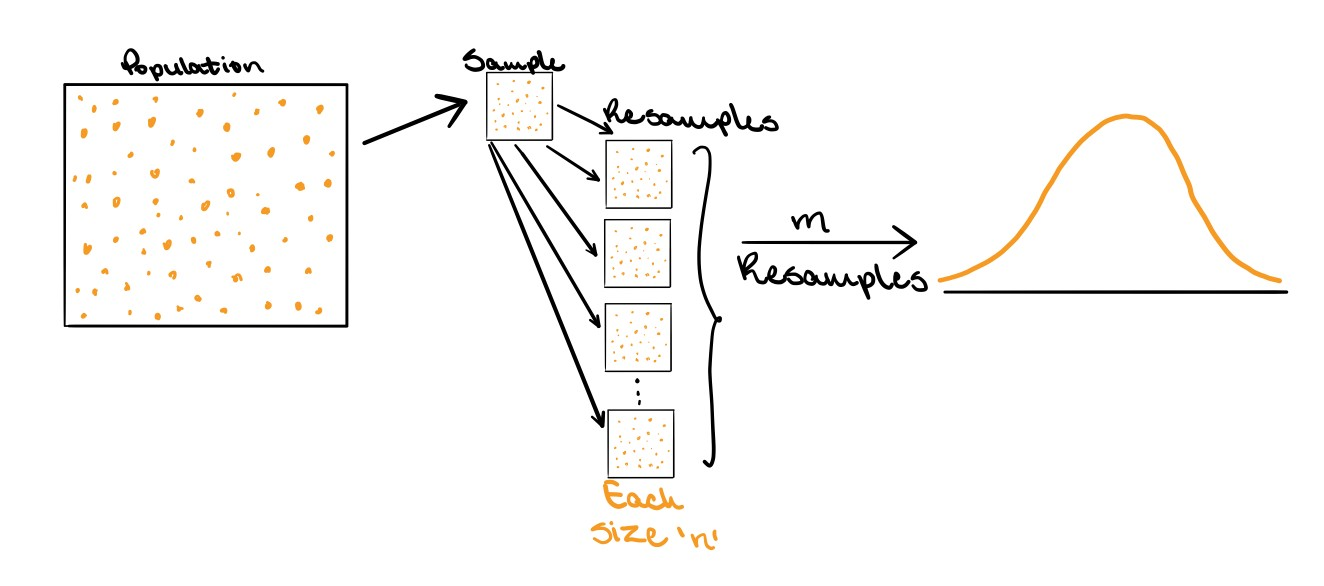
\includegraphics[width=0.7\textwidth]{figures/stats/bootstrapping.jpeg}
\caption{
Illustration of the bootstrapping method
by \href{https://towardsdatascience.com/bootstrapping-statistics-what-it-is-and-why-its-used-e2fa29577307}{Trist'n Joseph}.
Note that the $m$ resamples are done with replacement.
The final bootstrapped distribution is built by measuring the statistic in question on all of the bootstrapped samples,
and can be used to estimate the statistic's uncertainty.
}
\label{fig:bootstrapping}
\end{figure}

%%%%%%%%%%%%%%%%%%%%%%%%%%%%%%%%%%%%%%%%%%%%%%%%%%%%%%%%
\subsection{Hypothesis Testing}
\label{stats:bootstrapping:hypo}

As we can construct confidence intervals, bootstrapping can also be used for hypothesis testing.
{\Naive}ly we can test the null hypothesis by checking if the value in question,
typically \num{0}, lands within the confidence interval or not.
We can also estimate the \pvalue of a parameter by shifting the original sample distribution such that
it satisfies the null hypothesis, \eg shift all the data points by $\delta$ such that the sample has $\expval{x} = \num{0}$.
We then bootstrap the shifted sample to produce the bootstrapped distribution as normal.
The \pvalue is then the proportion of the bootstrapped distribution
with values differing from the null hypothesis by the observed difference or more,
\eg $P\left(\delta \leq \abs{x}\right)$ in the prior example.

%%%%%%%%%%%%%%%%%%%%%%%%%%%%%%%%%%%%%%%%%%%%%%%%%%%%%%%%
\subsection{Poisson Bootstrapping}
\label{stats:bootstrapping:poisson}

For large sample sizes $n$, instead of drawing $m$ bootstrap samples with replacement,
which can be computationally expensive,
we can use the single sample,
but give each data point a weight $w$ drawn
from the Poisson distribution with $\lambda = 1$.
The set of weights is then generated $m$ times.
Formally, the methods are equivalent as for large $n$
the binomial probability of including a given data point approaches the Poisson probability with $\lambda = 1$.
Poisson bootstrapping is commonly used in particle physics,
in particular see the direct balance $\gamma\text{+Jet}$ calibration
in the dissertation \cite{mepland_dissertation}, Appendix E.1.4.

%%%%%%%%%%%%%%%%%%%%%%%%%%%%%%%%%%%%%%%%%%%%%%%%%%%%%%%%
%%%%%%%%%%%%%%%%%%%%%%%%%%%%%%%%%%%%%%%%%%%%%%%%%%%%%%%%
\section{Bayesian Statistics}
\label{stats:Bayes}
% TODO

% \cref{stats:Bayes_rule}

%%%%%%%%%%%%%%%%%%%%%%%%%%%%%%%%%%%%%%%%%%%%%%%%%%%%%%%%
\subsection{Bayesian Conjugate Prior}
\label{stats:Bayes:conjugate_prior}
% TODO

%%%%%%%%%%%%%%%%%%%%%%%%%%%%%%%%%%%%%%%%%%%%%%%%%%%%%%%%
\subsection{Bayes Estimator}
\label{stats:Bayes:estimator}
% TODO

%%%%%%%%%%%%%%%%%%%%%%%%%%%%%%%%%%%%%%%%%%%%%%%%%%%%%%%%
\subsection{Approximate Bayesian Computation (ABC)}
\label{stats:Bayes:ABC}
% TODO

%%%%%%%%%%%%%%%%%%%%%%%%%%%%%%%%%%%%%%%%%%%%%%%%%%%%%%%%
%%%%%%%%%%%%%%%%%%%%%%%%%%%%%%%%%%%%%%%%%%%%%%%%%%%%%%%%
\section{Bias of a Predictor}
\label{stats:bias}
% TODO

\begin{equation}\label{eq:stats:bias}
\bias{\hat{f}\left(x\right)} = \expval{\hat{f}\left(x\right)} - f\left(x\right)
\end{equation}

%%%%%%%%%%%%%%%%%%%%%%%%%%%%%%%%%%%%%%%%%%%%%%%%%%%%%%%%
%%%%%%%%%%%%%%%%%%%%%%%%%%%%%%%%%%%%%%%%%%%%%%%%%%%%%%%%
\section{Kullback-Leibler Divergence}
\label{stats:kld}
% TODO

%%%%%%%%%%%%%%%%%%%%%%%%%%%%%%%%%%%%%%%%%%%%%%%%%%%%%%%%
%%%%%%%%%%%%%%%%%%%%%%%%%%%%%%%%%%%%%%%%%%%%%%%%%%%%%%%%
\section{Markov Chains}
\label{misc:markov_chains}
% TODO

%%%%%%%%%%%%%%%%%%%%%%%%%%%%%%%%%%%%%%%%%%%%%%%%%%%%%%%%
%%%%%%%%%%%%%%%%%%%%%%%%%%%%%%%%%%%%%%%%%%%%%%%%%%%%%%%%
\section{Markov Chain Monte Carlo (MCMC)}
\label{misc:MCMC}
% TODO

% Markov Chain Monte Carlo (MCMC) is a Monte Carlo (MC) method

%%%%%%%%%%%%%%%%%%%%%%%%%%%%%%%%%%%%%%%%%%%%%%%%%%%%%%%%
\subsection{\pymcThree}% would rather have the \textsc caps than italics
\label{misc:MCMC:PyMC3}
% TODO
% TODO \pymcThree

%%%%%%%%%%%%%%%%%%%%%%%%%%%%%%%%%%%%%%%%%%%%%%%%%%%%%%%%
%%%%%%%%%%%%%%%%%%%%%%%%%%%%%%%%%%%%%%%%%%%%%%%%%%%%%%%%
\section{Sampling from Probability Distributions}
\label{misc:sampling_prob_dist}

Most programming languages have built-in functions to generate
pseudo-random numbers from common probability distributions,
such as the Poisson \cref{eq:stats:poisson:P} or Gaussian \cref{eq:stats:gaus:P} distributions.
However, in some cases we may wish to sample from an unsupported esoteric function.
In these situations we can turn to inverse transform sampling and rejection sampling,
to give just two examples from many possible computational methods,
to construct the desired distribution from an existing random number generator.

%%%%%%%%%%%%%%%%%%%%%%%%%%%%%%%%%%%%%%%%%%%%%%%%%%%%%%%%
\subsection{Inverse Transform Sampling}
\label{misc:sampling_prob_dist:inverse}
% https://www.youtube.com/watch?v=9ixzzPQWuAY

If we know the explicit form of the target probability density function (PDF), $X = P\left(x\right)$,
can integrate it to find the cumulative distribution function (CDF), $F_{X}\left(x\right) = \int_{-\infty}^{x} P\left(t\right) \, \dd{t}$,
and furthermore can invert the CDF\footnote{The inverse CDF
is known as the percent point function, \texttt{ppf},
in \href{https://docs.scipy.org/doc/scipy/reference/stats.html}{\scipy}.}, $F^{-1}_{X}\left(u\right)$ for $0 \leq u \leq 1$,
we can explicitly transform the uniform distribution $U\left(x\right)$ into $P\left(x\right)$ as:

\begin{equation}\label{eq:stats:sampling_prob_dist:inverse}
F^{-1}_{X}\left(U\right) = P\left(x\right) = X\,.
\end{equation}

To prove the method, assuming that $F^{-1}_{X}$ exists, we can do:

\begin{subequations}\label{eq:stats:sampling_prob_dist:inverse_proof}
\begin{align}
P\left(F^{-1}_{X}\left(U\right) \leq x\right) &= P\left(U \leq F_{X}\left(x\right) \right) \label{eq:stats:sampling_prob_dist:inverse_proof:inverse} \\
&= F_{X}\left(x\right)\,,\label{eq:stats:sampling_prob_dist:inverse_proof:def} \\
P\left(U \leq y\right) &= y\,, \label{eq:stats:sampling_prob_dist:inverse_proof:U}
\end{align}
\end{subequations}

\noindent where in \cref{eq:stats:sampling_prob_dist:inverse_proof:inverse} we have applied $F$ to both sides of the inner inequality,
and in \cref{eq:stats:sampling_prob_dist:inverse_proof:def} we have used the definition of the uniform distribution \cref{eq:stats:sampling_prob_dist:inverse_proof:U}.
As $P\left(F^{-1}_{X}\left(U\right) \leq x\right) = F_{X}\left(x\right) = P\left(X \leq x\right)$
we can compare terms and see \cref{eq:stats:sampling_prob_dist:inverse}.

The inverse sampling method can be seen graphically \cref{fig:stats:sampling_prob_dist:inverse} being used to generate the normal distribution.

%\begin{figure}
%\centering
%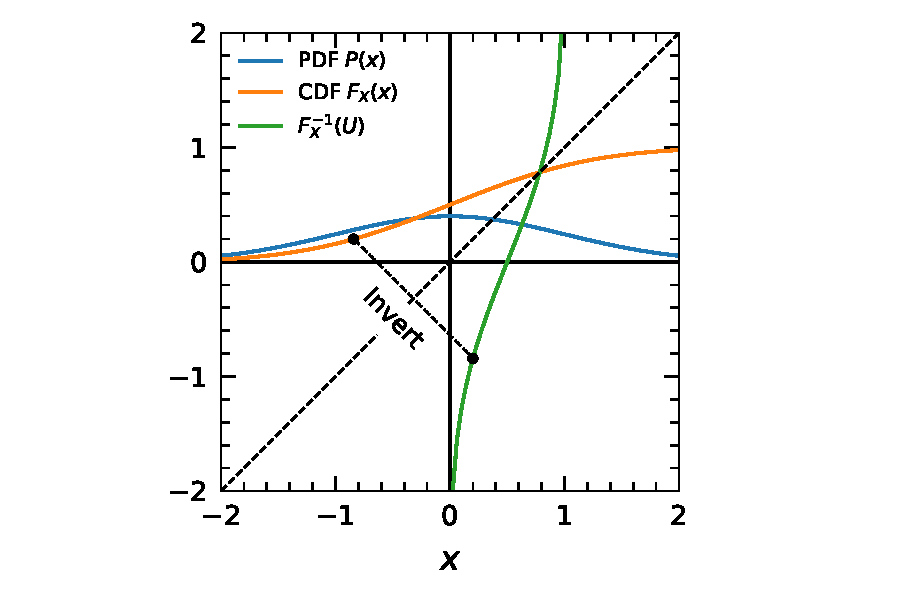
\includegraphics[width=0.7\textwidth]{figures/stats/inverse_transform_sampling_normal_dist}
%\caption{
%Example application of the inverse sampling method to generate the normal distribution, adapted from \href{https://en.wikipedia.org/wiki/File:Inverse_transform_sampling.png}{Olivier Ricou}.
%}
%\label{fig:stats:sampling_prob_dist:inverse}
%\end{figure}

%%%%%%%%%%%%%%%%%%%%%%%%%%%%%%%%%%%%%%%%%%%%%%%%%%%%%%%%
\subsection{Rejection Sampling}
\label{misc:sampling_prob_dist:reject}
% https://www.youtube.com/watch?v=OXDqjdVVePY

While inverse transform sampling is a computationally efficient method
its assumptions will not be met by all interesting PDFs,
in particular if we do not have an explicit, invertible CDF.
In these cases we can turn to rejection sampling instead,
which can handle more general PDFs at the cost of a lower computational efficiency.

In rejection sampling, we assume we know the PDF of the random variable to be sampled from,
up to a normalization constant $A$ \cref{eq:stats:sampling_prob_dist:reject:X}.
We then choose a different PDF, $g\left(x\right)$ which is easy for us to sample from.
Any $g\left(x\right)$ covering the range of $x$ will do,
but the method is more efficient the closer we can get $g\left(x\right)$ to match $f\left(x\right)$.
$g\left(x\right)$ is then scaled by a known constant $M$
such that it is always larger than $f\left(x\right)$ \cref{eq:stats:sampling_prob_dist:reject:f_condition}
as illustrated in \cref{fig:stats:sampling_prob_dist:reject}.
Finally, we sample random $x$ values from $g\left(x\right)$ and accept them with probability \cref{eq:stats:sampling_prob_dist:reject:P_accept}.
The accepted $x$ values will have the same distribution as $X$.

\begin{subequations}\label{eq:stats:sampling_prob_dist:reject}
\begin{align}
X = P\left(x\right) &= \frac{1}{A} f\left(x\right), \label{eq:stats:sampling_prob_dist:reject:X} \\
\forall x, \quad f\left(x\right) & \leq M g\left(x\right), \label{eq:stats:sampling_prob_dist:reject:f_condition} \\
P\left(\text{Accept} \mid x\right) &= \frac{f\left(x\right)}{M g\left(x\right)}\,. \label{eq:stats:sampling_prob_dist:reject:P_accept}
\end{align}
\end{subequations}

\begin{figure}[H]
  \centering
  \savebox{\largestimage}{
    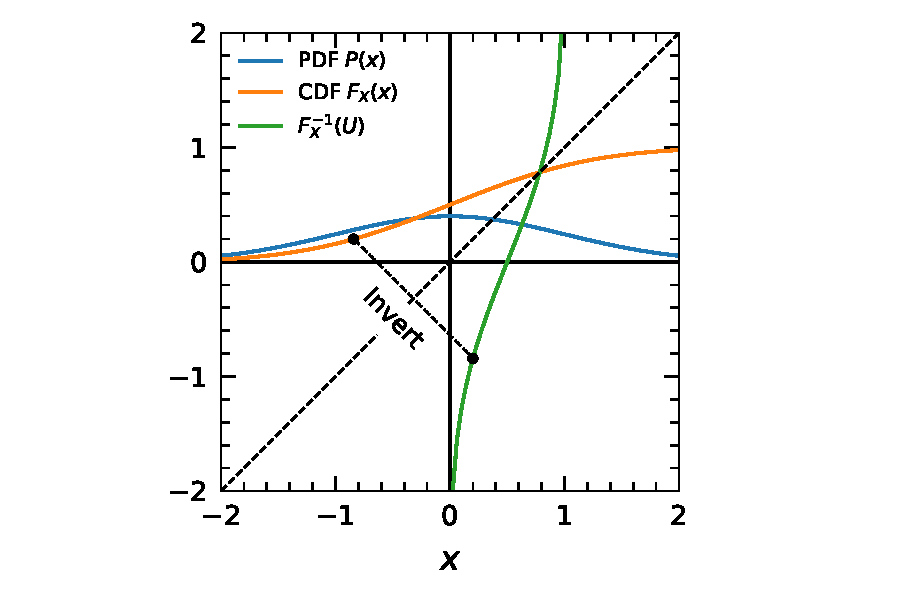
\includegraphics[width=0.47\textwidth,trim={3.0cm 0.5cm 3.0cm 0.1cm},clip]{figures/stats/inverse_transform_sampling_normal_dist}% trim={<left> <lower> <right> <upper>}
  }% Store largest image in a box

  \begin{subfigure}[b]{0.48\textwidth}\centering
    \usebox{\largestimage}
    \vspace{0.01cm}
  \caption{Inverse Sampling}
  \label{fig:stats:sampling_prob_dist:inverse}
  \end{subfigure}
  ~
  \begin{subfigure}[b]{\wd\largestimage}\centering
    \raisebox{\dimexpr.5\ht\largestimage-.5\height}{% Adjust vertical height of smaller image
      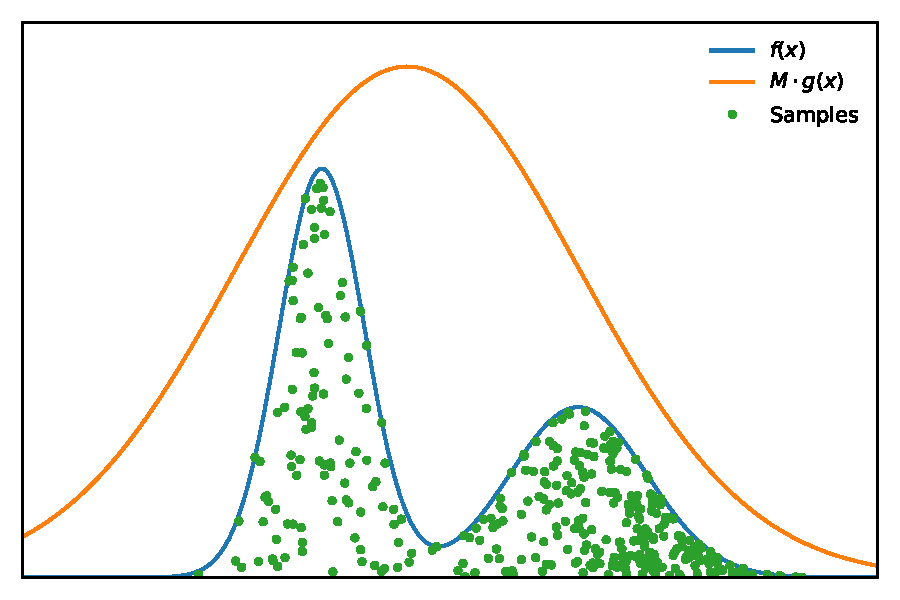
\includegraphics[width=\textwidth]{figures/stats/rejection_sampling}}
  \caption{Rejection Sampling}
  \label{fig:stats:sampling_prob_dist:reject}
  \end{subfigure}
\caption{
Illustrations of the inverse sampling and rejection sampling methods, adapted from \href{https://en.wikipedia.org/wiki/File:Inverse_transform_sampling.png}{Olivier Ricou} and \href{https://www.data-blogger.com/2016/01/24/the-mathematics-behind-rejection-sampling/}{Kevin Jacobs}.
  \label{fig:stats:sampling_prob_distr}
}
\end{figure}

For a proof of why the rejection sampling method works see \cref{eq:stats:sampling_prob_dist:reject:proof} below
which hinges on Bayes' Theorem from \cref{stats:Bayes_rule} in \cref{eq:stats:sampling_prob_dist:reject:proof:x_given_Accept}
along with other basic definitions from probability theory.

\begin{subequations}\label{eq:stats:sampling_prob_dist:reject:proof}
\begin{align}
P\left(x \mid \text{Accept}\right) &= \frac{P\left(\text{Accept} \mid x\right) P\left(x\right)}{P\left(\text{Accept}\right)} = \frac{1}{P\left(\text{Accept}\right)} \frac{f\left(x\right)}{M \cancel{g\left(x\right)}} \cancel{g\left(x\right)}, \label{eq:stats:sampling_prob_dist:reject:proof:x_given_Accept} \\
P\left(\text{Accept}\right) &= \int_{-\infty}^{\infty} P\left(\text{Accept} \mid x\right) g\left(x\right) \, \dd{x} \label{eq:stats:sampling_prob_dist:reject:proof:P_Accept1} \\
&= \int_{-\infty}^{\infty} \frac{f\left(x\right)}{M g\left(x\right)} g\left(x\right) \, \dd{x} = \frac{1}{M} \int_{-\infty}^{\infty} f\left(x\right) \, \dd{x} = \frac{A}{M}, \label{eq:stats:sampling_prob_dist:reject:proof:P_Accept2} \\
\implies P\left(x \mid \text{Accept}\right) &= \frac{f\left(x\right)/M}{A/M} = \frac{1}{A} f\left(x\right) = P\left(x\right) = X. \label{eq:stats:sampling_prob_dist:reject:proof:conclusion}
\end{align}
\end{subequations}

%%%%%%%%%%%%%%%%%%%%%%%%%%%%%%%%%%%%%%%%%%%%%%%%%%%%%%%%
\subsection{Metropolis-Hastings Algorithm}
\label{misc:sampling_prob_dist:metropolis_hastings}
% TODO
